\section{Persistence}

\begin{figure}[!htb]
    \centering
    \includegraphics[width=0.8\textwidth]{figures/DB Screenshot users.png}
    \caption{A document showcasing a user, in this case an admin, in the database}
    \label{fig:userDB}
\end{figure}

\begin{figure}[!htb]
    \centering
    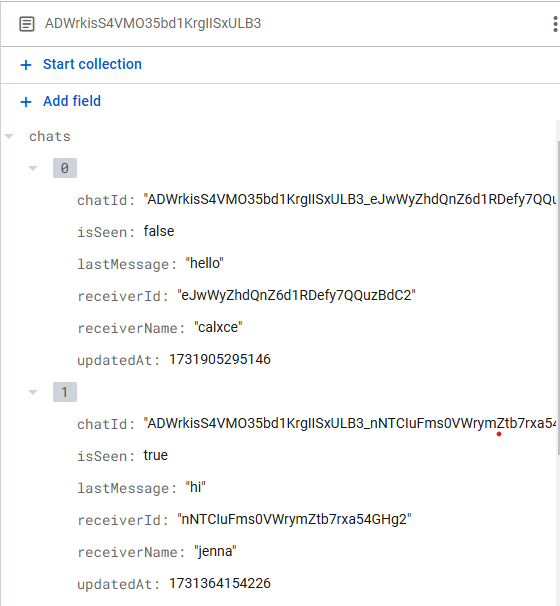
\includegraphics[width=0.8\textwidth]{figures/DB Screenshot userChats.png}
    \caption{A document showcasing a userChat in the database}
    \label{fig:userChatDB}
\end{figure}

\begin{figure}[!htb]
    \centering
    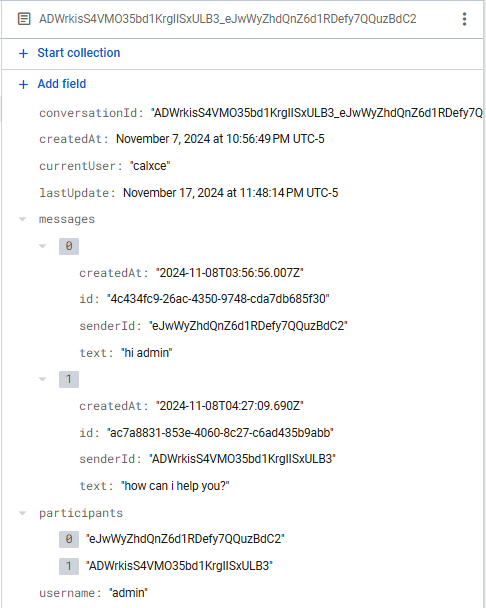
\includegraphics[width=0.8\textwidth]{figures/DB Screenshot conversations.png}
    \caption{A document showcasing a conversation in the database}
    \label{fig:conversationDB}
\end{figure}

\begin{figure}[!htb]
    \centering
    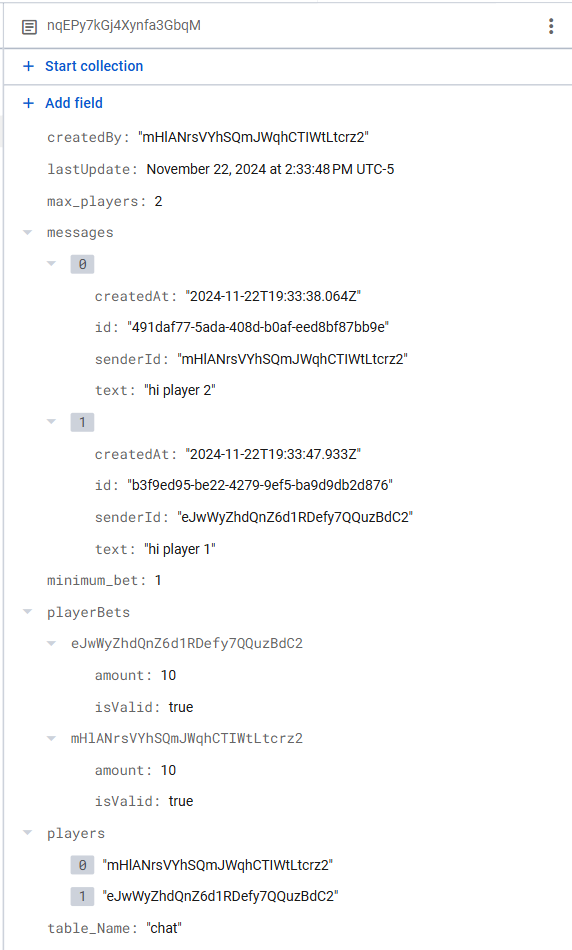
\includegraphics[width=0.7\textwidth]{figures/DB Screenshot table.png}
    \caption{A document showcasing a table in the database}
    \label{fig:tableDB}
\end{figure}

We used Firebase, a NoSQL database to store our persistent data. We created four collections: users, conversations, userChats, and table which maintained user data, messages among account owners, and table information. The users collection contained fields like email, first name, last name, user ID, username, a list of friends, total wins and losses, their chip balance, and a role which can either be an account user or admin. UserChats contained data that detailed the most recent updates of a conversation with another user. It included a chat ID, a Boolean isSeen to indicate whether the message was read, a receiver id, receiver name, the last message sent in the conversation, and a timestamp for when the last message was sent. The conversations collection managed the messages sent between two users. It stored the conversation ID, timestamps for when the conversation was initially created and of the latest update, and a list of participants which held the two users’ user IDs. The collection had a field called messages that was an array of maps. Each map contained fields for a message ID, the message content, the user ID of the sender, and a timestamp for when the message was created.

 The table collection managed information about the table as well as the current round being played. It saved the user ID of the host as the table creator, the table name, the user IDs of players sitting at the table, the table’s minimum bet, the max amount of players, and each player’s bet for the round. When a game was in session, the gameStarted Boolean was set to true. It also had the ID of the current player in the session, each individual’s hand which was an array of the suit, rank, and value of a card, the dealer’s hand, and the player’s statuses such as if they won the round, busted, or the dealer won. Table messages were stored in this collection in the same format as conversations.

 \clearpage
